\appendix

\section{Claims of the Earlier Evaluation}

\begin{table*}[t]
\centering
\footnotesize
\begin{tabular}{@{}p{0.40\textwidth}p{0.55\textwidth}@{}}
\toprule
Earlier claim \citep{rajan2025codexverify} & What the data shows \\
\midrule
76.1\% TPR and 68.7\% accuracy on 99 samples with verified labels. &
Reproduced exactly (\nOldCvTpr\% TPR, \nOldCvAcc\% accuracy). 70 samples were generated by Claude together with their labels; \nOldBugComments{} samples carry a \texttt{\# BUG} comment; always answering ``buggy'' scores \nOldMajority\%. On execution labels: AUC \nHefCvAuc{} (HumanEvalFix) and \nSweCvAuc{} (SWE-bench). \\
Catches as many bugs as Meta Prompt Testing (75\%) without test execution. &
The 75\% figure is reported on a different dataset. The Correctness agent executes the code it analyzes. \\
Combining agents with different detection patterns provably finds more bugs, by submodularity of mutual information under conditional independence. &
Only monotonicity of $I(A_S;B)$ holds without assumptions (\S\ref{sec:dependence}); it concerns information, not an aggregator's accuracy. Submodularity needs conditional independence, which the LLM agents violate (\S\ref{sec:dependence}). \\
Measured agent correlation $\rho=0.05$--$0.25$ confirms the agents detect different bugs. &
The released code computes no such correlation. Measured here: static agents $\rho$ \nStaticSweRhoMin{} to \nStaticSweRhoMax{} with \nStaticSweMiAll{} bits of label information; LLM agents $\rho$ \nSonnetSweRhoMin{} to \nSonnetSweRhoMax{} (Table~\ref{tab:corr}). \\
Multiple agents improve accuracy by 39.7 points (32.8\% to 72.4\%) with diminishing returns. &
An average over subsets of each size, dominated by subsets without the Correctness agent, on 29 samples with 5 correct ones. On execution labels all 15 subsets have AUC \nSweAblWorst--\nSweAblBest{} (Table~\ref{tab:ablation}). \\
Best pair, Correctness + Performance, reaches 79.3\% accuracy. &
On execution labels this pair has AUC \nHefAblCP{} on HumanEvalFix and \nSweAblCP{} on SWE-bench. \\
Paired Semgrep baseline: 4.8\% TPR, 28.6\% accuracy on the same samples. &
The released Semgrep run analyzed code from a different generation run than the main evaluation (0 of 28 samples identical). On paired execution-labeled data Semgrep's AUC is \nHefSemgrepAuc{} and \nSweSemgrepAuc, as uninformative as CodeX-Verify. \\
$\chi^2$ test against Codex, $p<0.001$. &
The released code runs no Codex baseline on these samples, so the test has no paired data. \\
300 Claude Sonnet 4.5 patches: 99\% FAIL, 17\,ms per patch. &
The released run analyzed SWE-bench Lite's human gold patches (\nLiteFail{} of \nLiteN{} FAIL; \nLiteSyntax{} with a CRITICAL parse issue). On SWE-bench Verified gold patches the system flags \nGoldCv\% (\nGoldCvFail\% FAIL). \\
The 50\% FPR comes from quality defects that do not change program output. &
On execution labels FPR equals TPR: the system's flags are independent of correctness. \\
\bottomrule
\end{tabular}
\caption{Each claim of the earlier evaluation of CodeX-Verify next to what the committed data and code show.}
\label{tab:claims}
\end{table*}

\section{Ablation and Generator Breakdown}

\begin{table}[h]
\centering
\footnotesize
\begin{tabular}{@{}l cc cc@{}}
\toprule
 & \multicolumn{2}{c}{HumanEvalFix} & \multicolumn{2}{c}{SWE-bench agent patches} \\
\cmidrule(lr){2-3}\cmidrule(lr){4-5}
Agents & AUC & TPR$-$FPR & AUC & TPR$-$FPR \\
\midrule
C & 0.51 & 0.0 & 0.49 & -1.2 \\
S & 0.50 & 0.0 & 0.52 & 4.6 \\
P & 0.50 & 0.0 & 0.49 & -1.4 \\
St & 0.50 & 0.0 & 0.50 & -0.5 \\
\midrule
C+S & 0.50 & 0.0 & 0.49 & -0.6 \\
C+P & 0.50 & 0.0 & 0.49 & -1.2 \\
C+St & 0.50 & 0.0 & 0.48 & -1.2 \\
S+P & 0.50 & 0.0 & 0.52 & 3.2 \\
S+St & 0.50 & 0.0 & 0.53 & 2.4 \\
P+St & 0.50 & 0.0 & 0.50 & 0.3 \\
\midrule
C+S+P & 0.50 & 0.0 & 0.48 & -0.6 \\
C+S+St & 0.50 & 0.0 & 0.49 & -0.6 \\
C+P+St & 0.50 & 0.0 & 0.49 & -1.2 \\
S+P+St & 0.50 & 0.0 & 0.52 & 0.9 \\
\midrule
C+S+P+St & 0.50 & 0.0 & 0.48 & -0.6 \\
\midrule
Shapley, C & +0.005 & & -0.024 & \\
Shapley, S & -0.000 & & +0.010 & \\
Shapley, P & -0.001 & & -0.005 & \\
Shapley, St & +0.000 & & +0.003 & \\
\bottomrule
\end{tabular}

\caption{CodeX-Verify agent subsets on execution-labeled data. AUC of the aggregator score and Youden's $J$ (TPR$-$FPR, \%) at the non-PASS flag. Shapley values decompose the full system's AUC gain over 0.5. C: Correctness, S: Security, P: Performance, St: Style.}
\label{tab:ablation}
\end{table}

\begin{table*}[t]
\centering
\footnotesize
\begin{tabular}{@{}l cccc@{}}
\toprule
 & \multicolumn{2}{c}{Claude 3.5 Sonnet agent (77 res./73 unres.)} & \multicolumn{2}{c}{GPT-4o Agentless (62 res./88 unres.)} \\
Verifier & AUC & Bal.\ acc. & AUC & Bal.\ acc. \\
\midrule
CodeX-Verify (FAIL or WARN) & 0.48 & 50.0 & 0.49 & 49.4 \\
CodeX-Verify, patch-aware & 0.53 & 53.1 & 0.54 & 54.3 \\
Haiku 5.5 single judge & 0.79 & 71.0 & 0.89 & 80.9 \\
Sonnet 5.5 single judge & 0.87 & 78.9 & 0.92 & 86.4 \\
Sonnet 5.5 4 agents, mean & 0.85 & 75.9 & 0.92 & 83.4 \\
\bottomrule
\end{tabular}

\caption{SWE-bench Verified results split by the agent that wrote the patch. Balanced accuracy in \%.}
\label{tab:generators}
\end{table*}

\begin{figure*}[t]
\centering
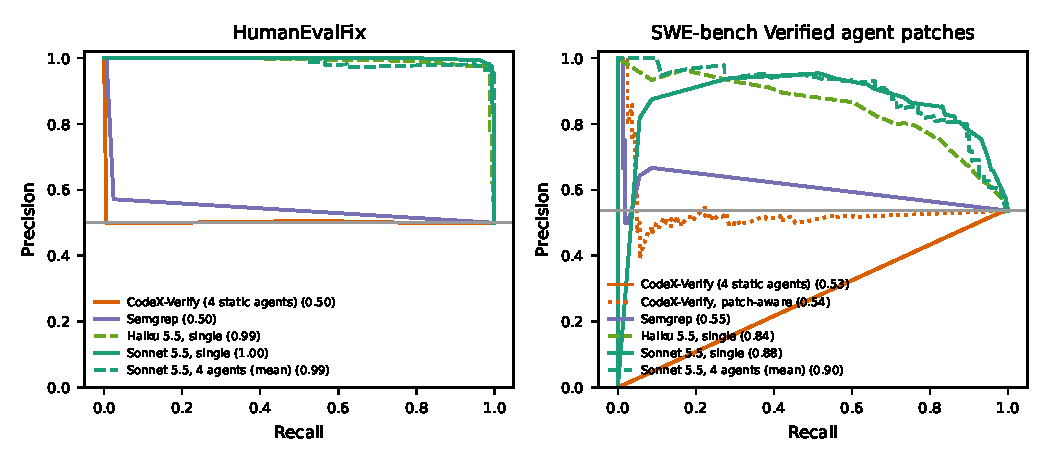
\includegraphics[width=0.85\textwidth]{figures/pr.pdf}
\caption{Precision--recall curves (average precision in parentheses). The horizontal line is the share of incorrect items.}
\label{fig:pr}
\end{figure*}

\section{Verifier Prompts and Settings}
\label{app:prompts}

All LLM calls use the system prompt ``You are an expert Python code reviewer acting as a pre-merge verifier. You cannot run the code. Answer with the JSON object requested.'', structured JSON output with fields \texttt{reason}, \texttt{p\_defect} (0--100), and \texttt{verdict} (ACCEPT/REJECT), and reasoning effort \texttt{low}. The user message starts with a focus line, then the item. Focus lines:
\begin{itemize}
\item single: ``Judge overall correctness: does the code do what it is supposed to do, for all valid inputs, without introducing problems?''
\item correctness: ``Focus only on functional correctness: logic errors, wrong results, off-by-one errors, unhandled edge cases, wrong exception behaviour.''
\item security: ``Focus only on security: injection, unsafe deserialization, secrets, path traversal, unsafe use of eval/exec/subprocess, and other vulnerabilities.''
\item performance: ``Focus only on performance: algorithmic complexity, unnecessary work, resource leaks, scalability problems.''
\item style: ``Focus only on maintainability and style: readability, naming, structure, documentation, code smells.''
\end{itemize}
For HumanEvalFix the item is the function with the instruction to decide whether the implementation satisfies its docstring. For SWE-bench it is the issue text and the patch, with the instruction that the patch should resolve the issue without breaking existing behaviour and that hidden tests will be run on it. The exact strings are in \texttt{bench/run\_llm.py}.

CodeX-Verify was run from the released source with its default configuration. In snippet mode it receives the added and context lines of the patch's Python hunks (capped at 30,000 characters) and the context flags the earlier evaluation used. In patch-aware mode it receives each touched file in full before and after the patch.

\section{Reproducibility}

\texttt{bench/build\_heval.py} and \texttt{bench/build\_swe.py} rebuild the benchmark from public sources (HumanEvalPack on Hugging Face; SWE-bench Verified; the two leaderboard submissions' predictions and \texttt{results.json}). \texttt{bench/run\_static.py}, \texttt{bench/run\_sast.py}, and \texttt{bench/run\_llm.py} produce the verifier outputs, which are committed under \texttt{results/rebuild/}. \texttt{bench/analyze.py} computes every table, figure, and in-text number of this paper from those outputs; in-text numbers are LaTeX macros it writes. \texttt{bench/robustness.py} computes the recall, stacking, permutation, and Holm analyses, and \texttt{bench/old\_set\_leak.py} reproduces Section~\ref{sec:v1}. Logged LLM calls cost \$\nCostUsd{} at list prices.
